\documentclass[draft]{agujournal2018}
\usepackage{apacite}
\usepackage{url} %this package should fix any errors with URLs in refs.
%\usepackage{lineno}
\linenumbers


\drafttrue
%\draftfalse
\journalname{JGR: Earth Surface}

%% you probably have to kill these custom commands later %% 
\newcommand\be{\begin{equation}} % shortcut to start eq envs 
\newcommand\ee{\end{equation}}   % shortcut to end eq envs
\newcommand\bra{\langle}
\newcommand\ket{\rangle}
\usepackage{amsmath,amssymb,amsfonts,amsthm}
\usepackage{comment}
\usepackage{wrapfig}
\usepackage{lipsum}
\usepackage{booktabs} % for wrapping text around tabulars in accord with
% https://tex.stackexchange.com/questions/49300/wrap-text-around-a-tabular
\usepackage{ragged2e}
\justifying

\begin{document}

\title{Joint stochastic theory of bedload transport and bed elevations: derivation of heavy-tailed resting times}
\authors{James K. Pierce\affil{1}\thanks{Vancouver, British Columbia, Canada}, and Marwan A. Hassan\affil{1}}
\affiliation{1}{Department of Geography, University of British Columbia}
\correspondingauthor{James K. Pierce}{kpierce@alumni.ubc.ca}

\begin{keypoints}
\item We model fluvial bedload activity and local bed elevation as a two-species stochastic birth-death process.
\item Computations show heavy-tailed power-law distributions of resting times for sediment undergoing burial, with universal tail parameters $\alpha=1.15$.
\item We discuss implications for bedload diffusion and suggest a new theoretical framework to approach the problem.

\end{keypoints}

\begin{abstract}
A consensus has formed that fluvial bedload resting times lie on heavy-tailed statistical distributions which may result from sediment burial.
However, due to observational difficulties, only a handful of experiments have resolved these distributions, and there have been few theoretical attempts to build understanding, leaving their generating mechanism and specific characteristics uncertain.
With reference to these issues, we present a new theory describing bedload transport and bed elevation changes as a joint stochastic process, deriving resting time distributions for sediment undergoing burial from the joint dynamics.
Our theory predicts heavy-tailed power-law distributions of resting times with universal tail behavior completely characterized by the mean erosion rate and its scaling with bed elevation changes.
\end{abstract} 

\section{Introduction}

% bulk transport vs. individual grains & relevance of research
The majority of classic studies into fluvial sediment transport have attempted to relate the bulk downstream flux of bedload to characteristics of the hydraulic forcing \citep[e.g.][]{Yalin1972}, yet the relevance of this approach to environmental problems is limited, as many contemporary issues require knowledge of differences between motions of individual grains, and not just average characteristics.
For example, the export of contaminants from channels \citep[e.g.][]{Malmon2005} and the morphological response of channels to ecological restoration efforts \citep[e.g.][]{Gaeuman2017} or changes in hydrology or sediment supply \citep[e.g.][]{Hassan2017} are not described by bulk fluxes, highlighting individual sediment motions as an important topic for geophysics research.

A significant complication is that individual grains transport within a noisy environment, which noise sources ranging across spatial and temporal scales from fluid turbulence \citep{Celik2014} and the variable arrangement of bed surface grains \citep{Gordon1972}, to channel morphology changes \citep{Hassan2017} and unsteady flows \citep{Phillips2013}.
As a result, the transport characteristics of individual grains are not deterministic \citep[e.g.][]{Einstein1937}, even in the most controlled laboratory experiments \citep[e.g.][]{Charru2004, Bohm2004, Fathel2015, Heyman2016}.

This led researchers to create probabilistic theories of individual motions based on random walk concepts, whereby bedload motions are approximated as alternating sequences of steps and rests, with step lengths and resting times treated as random variables associated with statistical distributions \citep{Einstein1937, Yano1969, Nakagawa1976, Hassan1991, Bradley2012}.
In these theories, differences between the random motions of one grain and the next imply bedload diffusion, or a spreading apart of grains as they transport.
The diffusion characteristics predicted by these models critically differ depending on whether the step length and resting time distributions have light or heavy tails \citep[e.g.][]{Bradley2017}.

Heavy-tailed distributions have exceedance functions $P(X>x) \sim x^{-\alpha}$ with tail parameters $\alpha < 2$, meaning large values of $x$ are relatively common, while light-tailed distributions have $\alpha \geq 2$, meaning large values of $x$ are relatively rare.
If both resting time and step distance distributions have light tails, the diffusion is said to be normal or Fickian, with a variance of particle positions $\sigma_x^2$
scaling with time $t$ as $\sigma_x^2 \propto t$.
However, if either distribution has a heavy-tail, the diffusion is called anomalous, with a variance of particle position scaling as $\sigma_x^2 \propto t^\gamma$, where $\gamma\neq 1$.
In this expression, $\gamma <1$ is called sub-diffusion and $\gamma > 1$ is super-diffusion.
In strongly asymmetric random walks such as bedload transport, heavy-tailed step lengths imply super-diffusion, while heavy-tailed resting times imply either super or sub-diffusion, depending on $\alpha$ \citep{Weeks1996, Weeks1998}.

Tracer experiments in gravel bed rivers show anomalous bedload diffusion \citep{Phillips2013, Bradley2017}, light-tailed step lengths \citep{Bradley2012, Hassan2013}, and heavy-tailed resting times \citep{Voepel2013, Olinde2015, Pretzlav2016, Bradley2017}, forming a coherent experimental picture of super-diffusive bedload transport, at least at long observation timescales \citep[e.g.][]{Nikora2002, Martin2012}.
However, field studies have not resolved the mechanism generating these heavy-tailed resting times \citep[e.g.][]{Bradley2017}, and empirical distributions display clear differences in their form and characteristics, showing different tail parameters \citep[e.g.][]{Olinde2015} and sometimes truncation \citep[e.g.][]{Bradley2017} or tempering to light tails at large resting times \citep[e.g.][]{Voepel2013}.
The mechanism generating heavy tails and these differences deserve attention.

A predominant hypothesis is that heavy-tailed resting times and anomalous diffusion originate from sediment burial \citep{Voepel2013,Martin2014,Wu2019}.
Conceptually, when grains rest on the bed surface, material transported from upstream can deposit on top of them, preventing entrainment until it's removed, driving up resting times and imparting a heavy tail to the distribution.
\citet{Martin2014} have provided the only direct support for this hypothesis.
They traced grains in a narrow flume with clear sidewalls, directly resolving burial as the generator of heavy-tailed resting times, and they described their results with a theoretical model, formally similar to an earlier effort by \citet{Voepel2013}.

The models of \citet{Voepel2013} and \citet{Martin2014} treat bed elevations as a random walk and interpret resting times as return periods from above in the bed elevation time-series \citep[e.g.][]{Redner2007}.
Both models are successful in describing different experimental resting time distributions.
However, the assumptions and results of these models are inconsistent with one another, and their treatment of bed elevations as a process independent of sediment transport is questionable, since erosion and deposition are the source of bed elevation changes \citep[e.g.][]{Wong2007}, suggesting further study is necessary.

In this work, we approach the problem from a different angle, making an extension of the stochastic bedload transport theory of \citet{Ancey2008} to link bed elevation changes to the erosion and deposition events of individual grains, and we derive resting times as a consequence of this theory.
The key assumptions of our model are: (1) bedload erosion and deposition can be characterized by probabilities per unit time, or rates \citep[e.g.][]{Einstein1950, Ancey2008}; and (2) these rates are contingent on the local bed elevation, encoding the property that erosion of sediment is emphasized from regions of exposure, while deposition is emphasized in regions of shelter \citep[e.g.][]{Sawai1987, Wong2007}.
Our theory generates heavy-tailed distributions with no tempering and a universal tail parameter $\alpha = 1.15$ for a particular non-dimensionalization of the resting time, showing close correspondence to the results of \citet{Martin2014} and suggesting a correction to some imperfections in their results.
We conclude the paper by framing our work in relation to earlier ideas and discussing the implications of this work on questions of individual bedload motions and anomalous diffusion.

\section{Stochastic theory}
\label{sec:theory}

% describe the set up 
We define a volume of downstream length $L$ which contains some number $n$ of moving particles in the water flow and some number $m$ of stationary particles composing the bed at some time $t$.
For simplicity, we consider all particles as approximately spherical with the same diameter $2a$, so their mobility and packing characteristics are similar.
Following \citet{Ancey2008}, we prescribe four events which can occur at any instant to modify the populations $n$ and $m$, and we characterize these events using probabilities per unit time, or rates.
These are: (1) migration of a moving particle into the volume from upstream ($n \rightarrow n+1$); (2) the entrainment of a stationary particle into motion within the volume ($m\rightarrow m-1$ and $n\rightarrow n+1$); (3) the deposition of a moving particle to rest within the volume ($m\rightarrow m+1$ and $n\rightarrow n-1$); and (4) the migration of a moving particle out of the volume to downstream ($n\rightarrow n-1$).
As the events occur at random intervals, they set up a joint stochastic evolution of the populations $n$ and $m$ characterized by a joint probability mass function (pmf) $P(n,m,t)$ having marginal pmfs $P(n,t) = \sum_m P(n,m,t)$ and $P(m,t) = \sum_n P(n,m,t)$ for the number of particles in motion and rest in the volume at $t$.
These concepts are depicted in figure \ref{fig:concept}.
\begin{figure}
  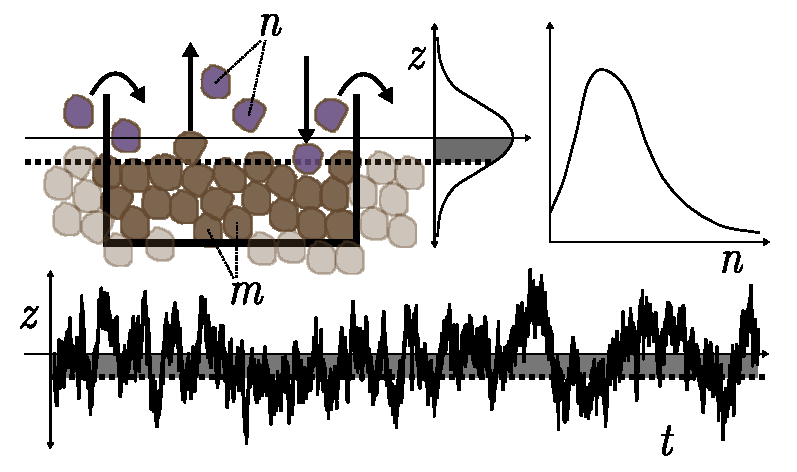
\includegraphics[width=\linewidth,keepaspectratio]{./figures/definition-combo.pdf}
  \vspace{-1.0cm}
  \caption{Definition sketch of a control volume containing $n$ moving grains and $m$ resting grains. Migration, entrainment, and deposition processes are represented by curved arrows, and the bed elevation at some instant is depicted by dotted line. The bed is presented in a degraded state, where $m<m_0$. The distributions of $n$ and $m$ are indicated in the upper right panel, while the bottom panel is a time-series of bed elevations (\ref{eq:ele}).}
  \label{fig:concept}
\vspace{-0.75cm}
\end{figure}

The populations $n$ and $m$ provide the bulk bedload flux $q_s$ and the local bed elevation $z$.
The mean bedload transport rate is given by $q_s \propto u_s \bra n \ket$, where $u_s$ is the characteristic velocity of moving bedload and $\bra n \ket = 
\sum_{n,m}nP(n,m) $ is the mean number of grains in motion \citep[e.g.][]{Charru2004, Ancey2008, Furbish2012a}.
The bed elevation is related to $m$ though the packing geometry of the bed.
To derive this, we prescribe a mean number of grains at rest $m_0$ and introduce a packing fraction $\phi$ of grains in the bed.
Then considering a two-dimensional bed \citep[e.g.][]{Einstein1950, Paintal1971}, the deviation from the mean bed elevation is
\be z(m) = \frac{\pi a^2}{\phi L}(m-m_0) = z_1(m-m_0). \label{eq:ele}\ee
The constant $z_1 = \pi a^2/(\phi L)$ is an important scale of the problem. 
$z_1$ is the magnitude of bed elevation change (in an average sense across the control volume) associated with the addition or removal of a single grain.
We write the rates of the four possible transitions as \citep[e.g.][]{Ancey2008}:
\begin{align}
 &R_{MI}(n+1,m|n,m) = \nu & \text{migration in}, \label{eq:rate1}\\
 &R_E(n+1,m-1|n,m) =\lambda(m) + \mu(m) n  & \text{entrainment},  \label{eq:rate2}\\
 &R_D(n-1,m+1|n,m) =\sigma(m) n & \text{deposition},\label{eq:rate3}\\
 &R_{MO}(n-1,m|n,m) =\gamma n & \text{migration out\label{eq:rate4}}.
\end{align}
These rates are independent of the past history of the populations and depend only on the current populations $(n,m)$. 
As a result, the system is Markovian \citep[e.g.][]{Cox1965, VanKampen1992}, meaning time intervals between subsequent transitions are exponentially distributed \citep[e.g.][]{Gillespie2007}.

In (\ref{eq:rate1}-\ref{eq:rate4}), $\nu$ and $\gamma$ are constants characterizing migration rates of individual grains into and out of the volume. 
They lack any dependence on the populations $n$ and $m$.
In contrast, $\lambda(m)$, $\mu(m)$, and $\sigma(m)$, characterizing the entrainment, collective entrainment \citep[e.g.][]{Ancey2008, Heyman2013, Heyman2014}, and deposition rates of individual grains are considered to depend on $m$.
As is well-known, bed elevation changes modify the likelihood of entrainment and deposition in a negative feedback \citep{Sawai1987, Wong2007}; that is, aggradation increases the likelihood of entrainment, while degradation increases the likelihood of deposition.
\citet{Wong2007} concluded that bed elevation changes induce an exponential variation in entrainment and deposition probabilities, while \citet{Sawai1987} concluded that the variation is linear.
For simplicity, we incorporate the scaling of \citet{Sawai1987} and note its equivalence to the \citet{Wong2007} scaling when bed elevation changes are small.
Because experimental distributions of bed elevations are usually symmetrical, \citep{Wong2007, Singh2009, Martin2014}, we expect the erosion and deposition feedbacks to be anti-symmetrical.
That is, as bed elevation changes drive up (down) erosion rates, so they drive down (up) deposition rates to the same degree.


% set up the m dependence of the rates
Summarizing these ideas, the entrainment and deposition rates can be written $\chi(m) = \chi_0(1\pm z_1 z(m)/(2l)^2)$, where $\chi = \lambda, \mu, \sigma$, and the entrainment parameters take the plus sign, while deposition takes the minus, and we have introduced a length scale $l$.
As we'll see, the variance of bed elevation turns out to be given by $\text{var}(z) = (l z_1)^2$. Accordingly, $l$ characterizes the range of bed elevation variations, which could be interpreted as the active layer depth \citep[e.g.][]{Church2017}.
Another perspective is that $l$ is the distance of bed elevation change at which the entrainment and deposition rates are significantly affected.
With these substitutions, the local bed elevation-dependent entrainment and deposition rates (\ref{eq:rate2}-\ref{eq:rate3}) can be written:
\begin{align}
R_E(n+1,m-1|n,m)&=[\lambda_0 + \mu_0 n]\Big[1 + \frac{z_1z(m)}{(2l)^2}\Big], && &\text{entrainment}, \label{eq:rate5}\\
R_D(n-1,m+1|n,m)&=\sigma_0 \Big[1-\frac{z_1z(m)}{(2l)^2}\Big]n, && &\text{deposition}. \label{eq:rate6}
\end{align}
At $z(m)=0$, the rates reduce to those of the \citet{Ancey2008} theory.
Away from this elevation, entrainment and deposition are alternatively suppressed and accentuated depending on the sign of $z(m)$.


In terms of the transition rates (\ref{eq:rate1}-\ref{eq:rate6}), we can obtain the Master equation for the probability flow using the forward Kolmogorov equation $\partial P(n,m;t)/\partial t = 
\sum_{n',m'} R(n,m)P(n',m';t)$ \citep[e.g.][]{Cox1965, Gillespie1992, Ancey2008} as 
\begin{multline}
 \frac{\partial P}{\partial t}(n,m;t) =  
\nu P(n-1,m;t) + 
\{\lambda(m+1) + [n-1]\mu(m+1)\}P(n-1,m+1;t)\\ + 
[n+1]\sigma(m-1)P(n+1,m-1;t) + 
[n+1]\gamma P(n+1,m;t) \\- 
\{ \nu + \lambda(m) + n\mu(m) + n\sigma(m) + n \gamma \}P(n,m;t).
 \label{eq:master}
\end{multline}
The joint probability distribution $P(n,m;t)$ solving this equation will fully characterize the statistics of $n$ and $m$.
We anticipate that solutions will adjust from the initial conditions to a steady-state distribution $P_s(n,m)$, independent of time, if the constant factors in the transition rates are representative of equilibrium bedload transport conditions.
This Master equation describes a two-species stochastic birth-death model \citep[e.g.][]{Cox1965} of a type well-known in the population ecology literature \citep[e.g.][]{Pielou1977, Swift2002}.
In our context, the two species are the moving and stationary grains in the volume.

\section{Numerical simulations}

Unfortunately, (\ref{eq:master}) does not appear to admit an analytical solution (but see \citet{Swift2002} for a standard method which fails in this case).
The difficulty stems from the product terms between $n$ and $m$.
In response, we resort to numerical methods, simulating (\ref{eq:master}) using the Gillespie algorithm \citep{Gillespie1977, Gillespie1992, Gillespie2007}.
The Gillespie algorithm leverages the defining property of a Markov process: when transition rates do not depend on the past, time intervals between transitions are exponentially distributed \citep[e.g.][]{Cox1965}.



\begin{wraptable}{l}{0.5\textwidth}
	\caption{Parameters from \citet{Ancey2008} experiments describing the rates of migration in, entrainment, deposition, and migration out when $z(m)=0$. All units are $s^{-1}$ (probability/time). Elevation changes modulate these rates in accord with (\ref{eq:ent}-\ref{eq:dep})}\label{tab:anceyparams}
	\begin{tabular}{cccccc} \\ 
		\toprule  
		Flow & $\nu$ & $\lambda_0$ & $\mu_0$ & $\sigma_0$ & $\gamma$ \\
		\midrule
		(a) & 5.45  & 6.59  & 3.74 & 4.67 & 0.77 \\
		\midrule
		(g) & 7.74  & 8.42  & 4.34 & 4.95 & 0.56 \\
		\midrule
		(i) & 15.56 & 22.07 & 3.56 & 4.52 & 0.68 \\
		\midrule
		(l) & 15.52 & 14.64 & 4.32 & 4.77 & 0.48 \\
		\midrule
		(n) & 15.45 & 24.49 & 3.64 & 4.21 & 0.36 \\
		\bottomrule
	\end{tabular}
\end{wraptable} 

Therefore, to step the Markov process through a single transition, it's enough to draw a random value from the exponential distribution of transition intervals to determine the time of the next transition.
Then, drawing another random value to choose the type of transition which occurs using the relative probabilities (\ref{eq:rate1}-\ref{eq:rate6}), the transition can be enacted by stepping $t,$, $n$ and $m$ by the appropriate shifts.
This procedure can be iterated to form an exact realization of the stochastic process \citep[e.g.][]{Gillespie2007}.

Using this algorithm, we simulated 5 flow conditions with 10 different values of $l$ taken across a range from $l=a$ (1 grain radius) to $l=10a$ (10 grain radii).
These values lie in the range exhibited in the majority of available experimental data \citep{Wong2007,Singh2009,Martin2014}.
For the migration, entrainment, and deposition parameters at each flow condition $(\nu, \lambda_0, \mu_0, \sigma_0, \gamma)$, we used values measured by \citet{Ancey2008} in a series of flume experiments.
These are summarized in table \ref{tab:anceyparams}.
Flow conditions are labeled (a), (g), and so on, roughly in order of increasing bedload flux (see \citet{Ancey2008} for more details). 
In all simulations, we take the packing fraction $\phi = 0.6$, a typical value for a pile of spheres \citep[e.g.][]{Bennett1972}, and set $L = 22.5cm$ and $a = 0.3 cm$, in accord with the \citet{Ancey2008} experiments.
Each simulation was run for $1500$hrs of virtual time, a period we selected by trial and error to ensure sufficient convergence of the statistics.

\section{Results}

Our simulations show intensely noisy time-series of bedload activities $n$, and temporally correlated bed elevation time-series (which can be seen in the bottom panel of figure \ref{fig:concept}).
From our chosen initial conditions, all simulations show a rapid attainment of steady state conditions followed by a stable stochastic dynamics of $n$ and $m$ which support a stable time-dependent probability $P_s(n,m)$. We compute this joint distribution by counting occurrences of the states $(n,m)$ in the simulated time series.
From this joint distribution we compute marginals $P(n)$ and $P(m)$ as explained in section \ref{sec:theory}.

Some of these marginal distributions are displayed in figure \ref{fig:pdfs}.
Neglecting changes in bed elevation, \citet{Ancey2008} analytically derived negative binomial (NegBin) distributions for the bedload activity $n$, and this functional form appears to be preserved through the coupling of their stochastic theory to bed elevation changes, with all of our computed distributions accepting clean NegBin fits.
For $m$, our computations obviously show Gaussian distributions, consistent with our assumptions about the scaling of erosion and deposition rates with bed elevation changes \citep[e.g.][]{Wong2007}.

\begin{figure}[t!]
	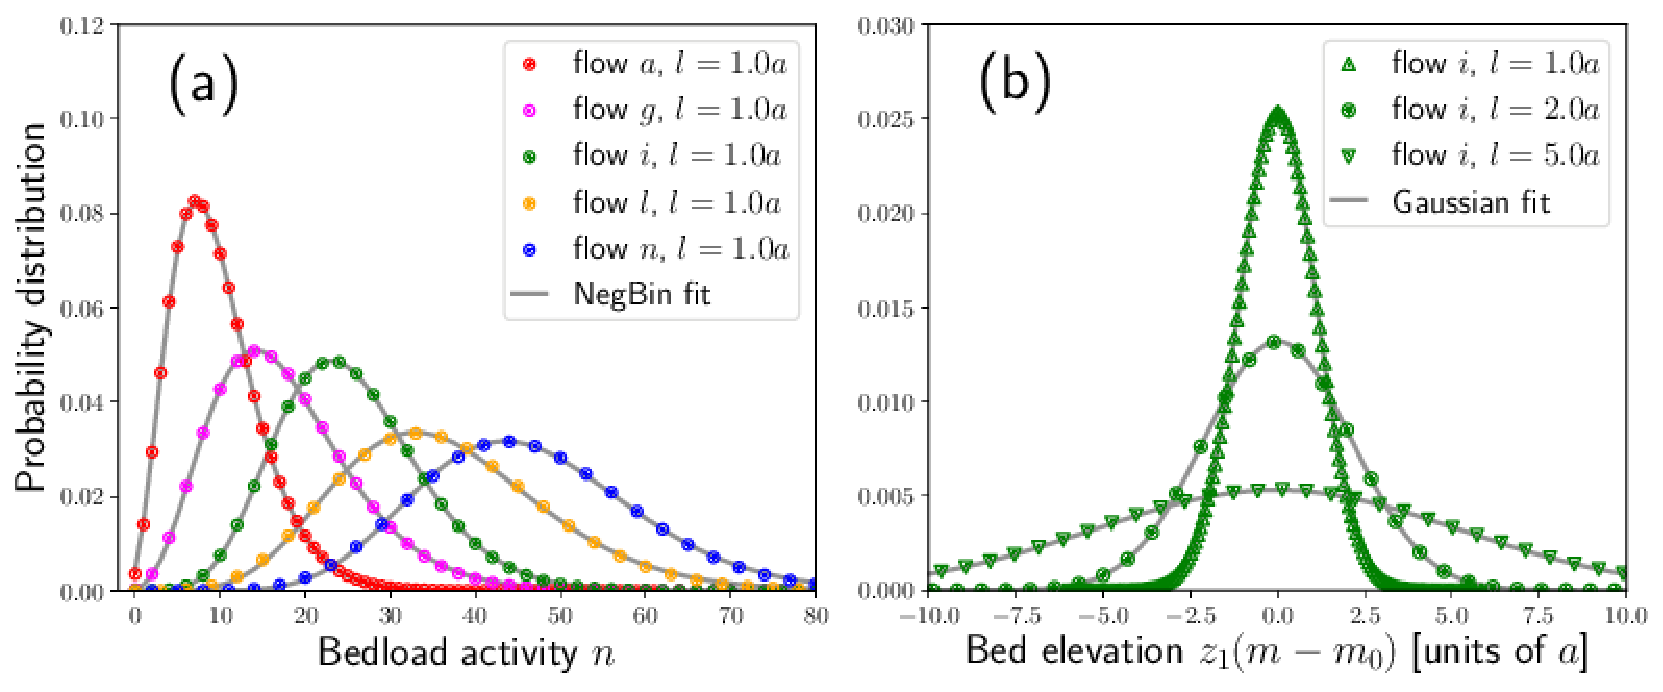
\includegraphics[width=\linewidth,keepaspectratio]{./figures/montage2.pdf}
	\caption{Marginal distributions for $n$ and $m$ for a small subset of simulations. Some points have been omitted for clarity.}
	\label{fig:pdfs}
\end{figure}

From the marginal distributions, we calculate means and variances of bedload activity and elevation ($m$).
The mean bed elevation is just the initial condition $m_0$. $m$ fluctuates around this value because it sets the equilibrium position of the elevation-related feedbacks in (\ref{eq:ele}).
The variance of $m$ appears given by $z_1^2 \text{var}(m) = l^2$, as indicated in figure \ref{fig:var}.
$l$ is a measure of bed elevation fluctuations.
The moments of $n$ are more difficult to understand.
Without dwelling on the issue, the moments of $n$ shift with the ratio $l/z_1$, somehow resulting from feedback between bed elevation changes and bedload transport.

\begin{wrapfigure}{r}{0.5\textwidth}
	\centering
	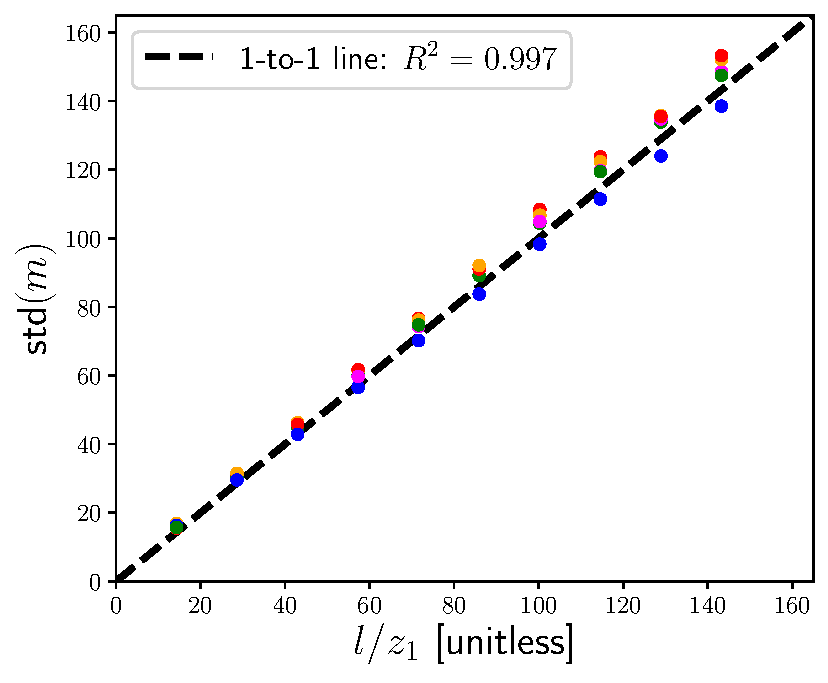
\includegraphics[width=0.5\textwidth,keepaspectratio]{./figures/variance.pdf}
	\caption{Data from all simulations is plotted to show that $l$ controls deviations of bed elevations: $l^2 = z_1^2\text{var}(m).$ We might interpret $l$ as the depth of the active layer \citep[e.g.][]{Church2017}.}
	\label{fig:var}
\end{wrapfigure}

Now we describe the analysis of bedload resting times from time-series of $m$.
Following \citet{Voepel2013} and \citet{Martin2014}, we concentrate on a particular bed elevation $m_\ast$, and find all time intervals separating deposition events at $m=m_\ast$ from erosion events at $m=m_\ast+1$.
Binning these return times to $m_\ast$ and counting the occurrences in each bin (using logarithmically spaced bins for presentation purposes), we obtain a non-exceedance distribution of return times $t_r$ held conditional to the elevation $m_\ast$: $P(T>t_r|m_\ast)$.
Using the marginal probability distribution of bed elevations, we derive the unconditional non-exceedance distribution of resting times as a sum over all elevations \citep{Yang1971, Nakagawa1980, Voepel2013, Martin2014}:
\be P(T>t_r) = \sum_{m'} P(m') P(T>t_r|m') .\ee
Some of these results are displayed in figure \ref{fig:cdfs}.
Comparing panels (a) and (c) shows the resting time distributions scale with flow condition and the standard deviation of bed elevation ($l$) differently.
However, as shown in panels (b) and (d), a characteristic timescale $T_0$ can collapse the tails of the distributions regardless.
\begin{figure}[t!]
	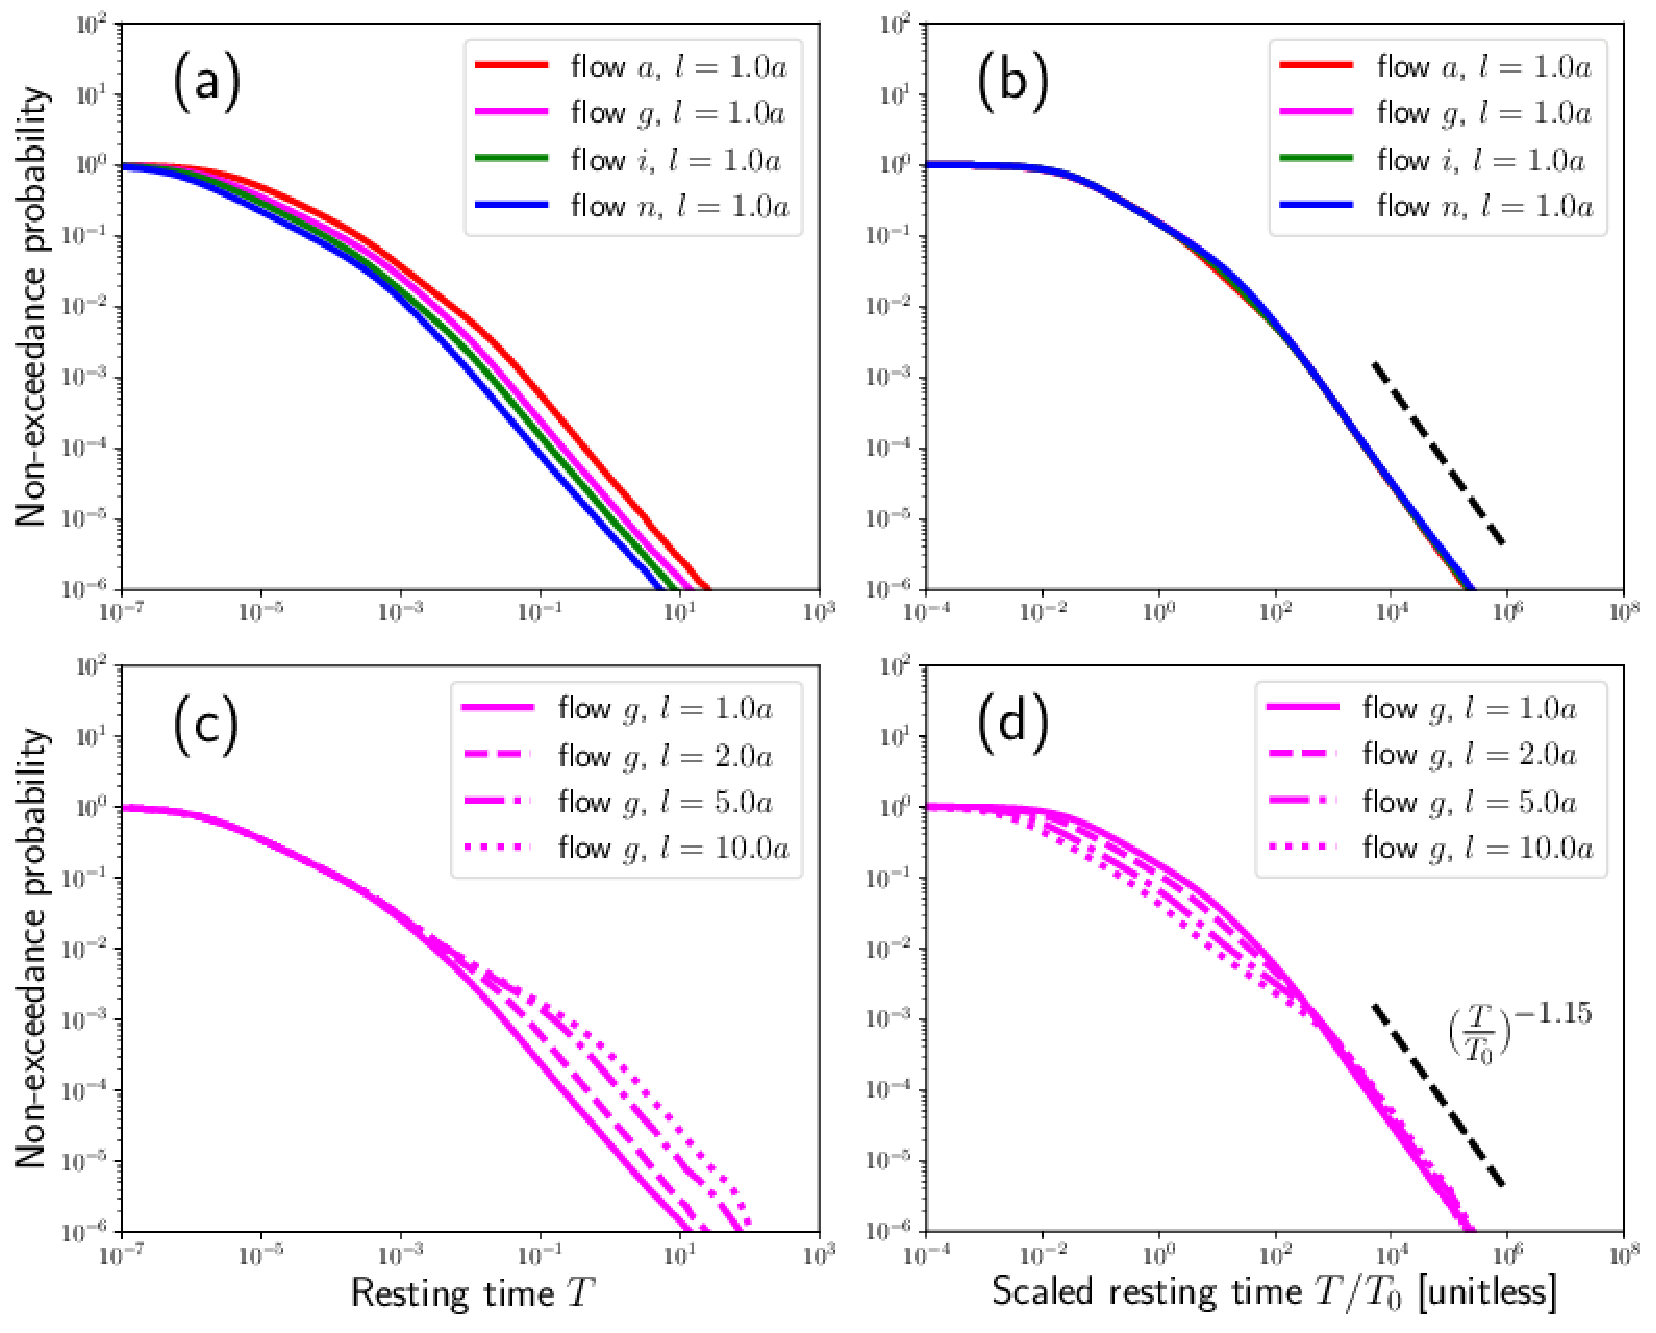
\includegraphics[width=\linewidth,keepaspectratio]{./figures/montage1.pdf}
	\caption{Resting time statistics vary in different ways with flow conditions and the variance of bed elevations. Panel (a) represents differing flow conditions at a fixed $l$ value, while panel (c) is fixed flow conditions at a variable $l$ value. When scaled by $T_0$ (\ref{eq:time}), both of types of difference collapse away in the tails of the distributions, as shown in panels (b) and (d). Finally, in panel (d), the black dotted line indicates a power law decay with tail parameter $\alpha=1.15$ .}
	\label{fig:cdfs}
\end{figure}

We can obtain $T_0$ heuristically by finding a characteristic velocity of bed elevation change.
Formally, the mean erosion rate is $E = \sum_{n,m}R_E(n,m)P(n,m)$.
This is the number of grains leaving the bed per unit time.
Since the removal of a single grain changes the bed elevation by $z_1$, bed elevations change with a characteristic velocity $z_1 E$.
Since the characteristic deviation of elevation is $l$, the time required for the bed to shift through a characteristic deviation is
\be T_0 = \frac{l}{z_1 E}.\label{eq:time}\ee
When scaling the resting time by $T_0$, we obtain the collapse of the distributions shown in figure \ref{fig:cdfs}.
As we see in the figure, for return times roughly satisfying $T/T_0 > 10^3$, all resting time non-exceedance distributions decay as a heavy-tailed power law with parameter $\alpha = 1.15$.

\section{Discussion}

Now we summarize our key results, relate them to previous work, and discuss their implications.
We have generalized the \citet{Ancey2008} bedload theory to include bed elevation changes, incorporating feedbacks between the local bed elevation and the instantaneous erosion and deposition rates \citep[e.g.][]{Wong2007}, forming a joint description of bedload transport and bed elevation changes. 
This model shows negative binomial distributions for the bedload activity and normal distributions for the bed elevation distribution, reproducing experimental results \citep{Ancey2008, Heyman2016, Wong2007, Singh2009,Martin2014}, and we've used it to derive resting time distributions of sediment undergoing burial, an object which is difficult to measure and not well understood \citep[e.g.][]{Voepel2013,Martin2014, Bradley2017}. 

Our joint theory (\ref{eq:master}) reduces to the independent descriptions of bedload by \citet{Ancey2008} and bed elevations by \citet{Martin2014} in certain cases, linking our approach to earlier work and providing some theoretical support for the mean-reverting random walk approach of \citet{Martin2014}.
Taking the limit $l\ll z_1$ obtains the theory of \citet{Ancey2008}.
In this case, we can neglect $z_1 z(m)/(2l)^2$ in comparison to $1$ in (\ref{eq:rate5}-\ref{eq:rate6}), and taking account of this change in (\ref{eq:master}), then summing over $m$, noting that $n$ and $m$ are independent in this limit, the master equation of \citet{Ancey2008} follows.
A master equation corresponding to the model of \citet{Martin2014} is obtained approximately from a mean-field approach.
Writing
\be n = \bra n \ket + \delta n \label{eq:mft}, \ee
where $\delta n$ are the fluctuations of $n$,  substituting this into (\ref{eq:master}) taking $m_0=0$ (without any loss of generality), then summing the resulting equations over $n$, gives
\be \frac{\partial}{\partial t}P(m,t) =  E \Big\{ \Big[1 +\Big(\frac{z_1}{2 l}\Big)^2m\Big]P(m+1,t) +  \Big[1 -\Big(\frac{z_1}{2 l}\Big)^2m\Big]P(m-1,t) - 2P(m,t)\Big\}, \label{eq:ou}\ee
neglecting all terms containing $\delta n$.
This is a discrete analog of the Ornstein-Uhlenbeck process \citep[e.g.][]{Gillespie1992}, the mean-reverting random walk used (in continuum form) by \citep{Martin2014}.
Differences between our bed elevation statistics and those predicted by (\ref{eq:ou}) are induced by $\delta n$.
Since the negative binomial distribution of $n$ has a wide tail, $|\delta n/\bra n \ket|$ has values often up to $3$ or $5$ \citep{Ancey2008}, so neglecting $\delta n$ is a crude approximation.
A deeper investigation into the differences between our bed elevation statistics and those of \citet{Martin2014} merit deeper investigation, but we won't dwell on this issue.
We note the theory of \citet{Voepel2013} is approached from a further limit $l\rightarrow \infty$ in (\ref{eq:ou}).
This limit is unphysical, since it implies bed elevation changes occur in the absence of coupling to bedload transport.
Accordingly, the bed elevation model of \citet{Voepel2013} is probably inappropriate and its conclusions on resting times questionable, although they first related the resting time to returns of the evolving bed --  a foundational contribution.

A possible generalization of our model is suggested by developments which followed the \citet{Ancey2008} bedload transport theory embedded in (\ref{eq:master}) \citep[e.g.][]{Ancey2014a, Heyman2014, Heyman2015}. 
These works are based on chaining many single-cell models from \citet{Ancey2008} together along a line, with migration out of one cell being migration in to another, and so on. 
These theories provide a framework to study spatial correlations in bedload transport.
One can imagine using our model (\ref{eq:master}) in the same way, chaining an array of them together along a line. This would generate a stochastic theory of 1D morphodynamics ultimately rooted in the foundational concepts of \citet{Einstein1950}.
An obvious issue with this idea is how to parameterize the entrainment and deposition rates of within the model in terms of the bed elevations.
Of course, this has been a longstanding issue in conventional 1D morphodynamics as well \citep[e.g.][]{Tucker2010}.

Finally, we discuss the computed resting time distributions (figure \ref{fig:cdfs}) and their properties, with special emphasis on the implications of these results for bedload diffusion.
Under the assumption of equilibrium bedload transport with a single grain size, we predict sediment burial generates heavy-tailed power law resting times with parameter $\alpha = 1.15$.
These tails collapse perfectly after scaling resting times by the factor $T_0 = l/(z_1 E)$, a characteristic timescale of bed elevation change.
We find asymptotic behaviors occur for $T/T_0>10^3$.
In contrast, \citet{Martin2014} scaled their distributions by an activity timescale they denoted as $1/a$, which is equivalent to $1/(2E)$.
Their scaling therefore contained no reference to the standard deviation of bed elevation $l$, which, as we mentioned, might be interpreted as an active layer thickness \citep{Church2017}.
\citet{Martin2014} acknowledged an imperfect collapse upon scaling their experimental resting time distributions. 
Our results suggest this may be corrected by scaling in addition by the active layer depth, which is expected to vary with transport stage \citep{Church2017}.


According to \citet{Weeks1998}, if the step length distribution has a light tail \citep[e.g.][]{Hassan2013}, our computed power-law resting times with tail parameter $\alpha = 1.15$ are sufficiently heavy-tailed to drive anomalous superdiffusion, scaling as $\sigma_x^2 \propto t^\gamma$ with $\gamma = 3 - \alpha = 1.85$.
In addition, since $1 \leq \alpha \leq 2$, tracer positions will have a convergent mean \citep[e.g.][]{Weeks1998, Bradley2017}.
For comparison, \citet{Martin2012} found $\alpha = 0.85$ from a three-dimensional flume experiment,  \citet{Voepel2013} found $\alpha = 0.88$ in data from the field study of \citet{Habersack2001},
\citet{Phillips2013} found $\alpha = 1.12$ from their field study, \citet{Martin2014} found $\alpha \approx 1.0$ from their simulations and two-dimensional flume experiments, and \citet{Bradley2017} found $\alpha = 0.67$ from field data. 
All of these values imply anomalous diffusion, like our simulation results, while only \citet{Phillips2013} and perhaps \citet{Martin2014} predict convergent means consistent with our results.
These discrepancies may stem from our assumption that burial is the source of heavy tails in these field data. 
We have analyzed return periods of the bed elevation, but as noted by \citet{Bradley2017}, 
other return periods impede tracer motions in gravel bed rivers, such as the deposition of sediment on top of floodplains \citep[e.g.][]{Bradley2013}, or on top of high bars in the bends of a stream \citep[e.g.][]{Bradley2017}.




\section{Conclusion}


Many open questions remain around the problem of anomalous bedload diffusion.
In this paper, we have made incremental steps forward, by framing sediment burial directly in terms of the sediment transport process.
When burial is a dominant process affecting the motions of individual grains, our results should serve as a prototype of this process, as they're derived under the assumptions of uniform grain size and equilibrium sediment transport in the spirit of \citet{Einstein1950}.
We predict anomalous bedload diffusion $\sigma_x^2 \propto t^{1.85}$ and a convergent mean, corroborating a subset of earlier studies.
Most directly, we have derived the \citet{Martin2014} model as an approximate limit of our more general theory, while we found no connection to the \citet{Voepel2013} model.
In closing, we highlight that other return processes in nature could impart heavy tails to fluvial bed material resting times \citep[e.g.][]{Bradley2017}.
To truly understand anomalous diffusion, we need to pin down these processes, quantify their relative importance, and learn to mix their effects.



\acknowledgments
The simulation code is available upon request from the first author. We would like to thank Shawn Chartrand and Conor McDowell for helpful discussions. 

\bibliography{biblio}

\end{document}




